\section{Fundamentals of optics}

In this chapter we will explore the physical nature of light and how we can use optical waveguides (microscopic "pipes") to trap and guide it over vast distances.

\subsection{Electromagnetic waves}

Light is an electromagnetic (EM) wave, it consists of an electric field and a magnetic field oscillating together. These two fields are orthogonal to each other, and they are both orthogonal to the direction the wave is traveling. For example, if a wave is moving directly away from you along the $z$-axis, the electric field might be oscillating up and down (the $y$-axis), wile the magnetic field oscillates left and right (the $x$-axis).

\begin{figure}[h!]
	\centering
	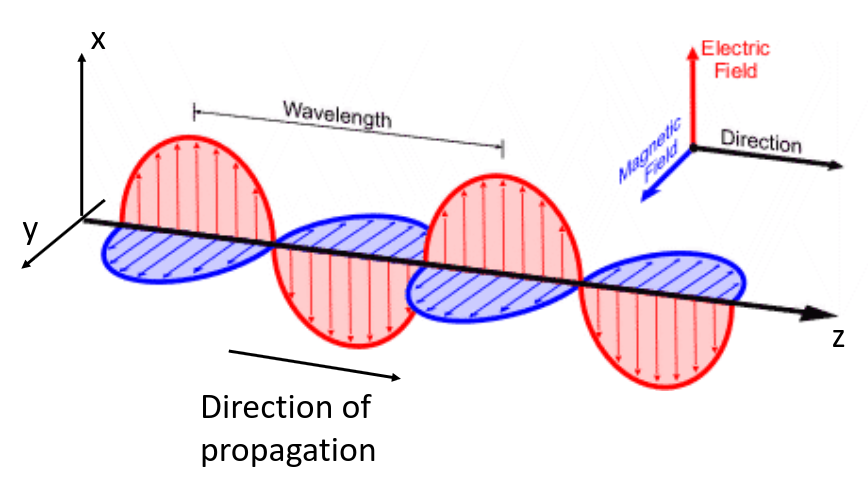
\includegraphics[width=0.6\textwidth]{images/em-wave-1}
    \caption{Electromagnetic wave}\label{fig:em-wave-1}
\end{figure}

To model a simplified, ideal EM wave in \textit{free space} (like a vacuum), we look at a \textit{monochromatic} wave (a wave with only a single frequency). The electric field $\vec E$ at a given position $(x, y, z)$ and time $t$ can be expressed by the \textbf{wave equation} as:
$$
\vec E(x, y, z, t) = \vec E_0 \cos (2 \pi f_0 t - Kz)
$$
where:
\begin{itemize}
    \item \textbf{Amplitude} $\vec E_0$ is the maximum strength of the electric field and the specific direction it is oscillating.
    \item \textbf{Frequency} $f_0$ is the number of oscillations per second, measured in Hertz (Hz). This is the inverse of the time period $T$.
    \item \textbf{Wave number} $K$ describes how the wave repeats in space, defined as $K = \frac{2\pi}{\lambda}$, where $\lambda$ is the spatial wavelength (as shown in Figure~\ref{fig:em-wave-1})
    \item \textbf{Phase} ($2 \pi f_0 t - Kz$). The negative sign here indicates that the wave is propagating forward along the $z$-axis. A positive sign would mean it is propagating backward.
    \item \textbf{Angular frequency} $\omega_0 := 2 \pi f_0$.
\end{itemize}

Note how the wave equation does not depend on $x$ or $y$. This is because the electric field's amplitude and phase are identical at every point across any infinitely large plane perpendicular to the $z$-axis. This makes it a \textbf{uniform plane wave}.

We can decompose the total electromagnetic field into the \textit{electric field} $\vec E$ and \textit{magnetic field} $\vec H$. Because space has three dimensions, any vector field can be decomposed into its components along the $x$, $y$, and $z$ axes:
$$
\vec E = E_x \hat i_x + E_y \hat E_y + E_z \hat i_z
$$
$$
\vec H = H_x \hat i_x + H_y \hat i_y + H_z \hat i_z
$$
where $\hat i_x$, $\hat i_y$, and $\hat i_z$ are the unit vectors pointing along the respective aces. This allows to calculate how a specific material boundary affects the horizontal and vertical part of the wave.

The electric and magnetic fields are fundamentally coupled. The direction of the wave's energy propagation is strictly determined by the cross product of the two fields $\vec E \times \vec H$. Moreover, their amplitudes are permanently locked together by the medium's \textbf{intrinsic impedance} $\eta$. If you know the vector of one field and the direction of propagation (let's call the unit vector of propagation $\hat i_k$), you can perfectly reconstruct one from the other:
$$
\vec H = \frac 1 \eta \left(\hat i_k \times \vec E \right)
\qquad
\vec E = - \eta \left(\hat i_k \times \vec H \right)
$$

